\documentclass[letterpaper]{article}

\usepackage{amsmath}
\usepackage{amssymb}
\usepackage{amsthm}
\usepackage{commath}
\usepackage{enumerate}
\usepackage{lmodern}
\usepackage{microtype}
\usepackage{fullpage}
\usepackage{graphicx}

\title{STAT 527: Assignment \#1}
\author{Philip Pham}
\date{\today}

\DeclareMathOperator{\E}{E}
\DeclareMathOperator{\Prob}{P}

\begin{document}
\maketitle

\section*{Problem 1}

\begin{enumerate}[(a)]
\item
  \begin{proof}
    This follows from the definition of variance after some algebra.
    \begin{align*}
      &\E\left[
      \left(\hat{f}(x) - f(x)\right)^2
        \right]
        = \E\left[
        \left[\left(\hat{f}(x) - \E\left[\hat{f}(x)\right]\right)
        +
        \left(\E\left[\hat{f}(x)\right] - f(x)\right)
        \right]^2
        \right] \\
      &=
        \E\left[\left(\hat{f}(x) - \E\left[\hat{f}(x)\right]\right)^2\right]
        +
        2\E\left[
        \left(\hat{f}(x) - \E\left[\hat{f}(x)\right]\right)
        \left(\E\left[\hat{f}(x)\right] - f(x)\right)
        \right]
        +
        \E\left[\left(\E\left[\hat{f}(x)\right] - f(x)\right)^2\right]
      \\
      &= \operatorname{var}\left(\hat{f}(x)\right)
	+ \left(\E\left[\hat{f}(x)\right] - f(x)\right)^2
        + 2\left(\E\left[\hat{f}(x)\right] - f(x)\right)\E\left[
        \left(\hat{f}(x) - \E\left[\hat{f}(x)\right]\right)        
        \right] \\
      &= \left(\E\left[\hat{f}(x)\right] - f(x)\right)^2 +
        \operatorname{var}\left(\hat{f}(x)\right).
    \end{align*}
  \end{proof}
\item
  \begin{proof}    
    The prediction error is
    \begin{align*}
      &\E\left[
      \left(y_{\text{new}} - \hat{f}\left(x_{\text{new}}\right)\right)^2
      \right]      
      = \E\left[
        \left(f\left(x_{\text{new}}\right) + \epsilon_\text{new} -
        \hat{f}\left(x_{\text{new}}\right)\right)^2
        \right] \\
      &= \E\left[
        \left(\epsilon_\text{new} +
        \left(f\left(x_{\text{new}}\right) -
        \hat{f}\left(x_{\text{new}}\right)\right)\right)^2
        \right] \\
      &= \E\left[\epsilon_\text{new}^2\right]
        + 2\E\left[\epsilon_\text{new}\left(f\left(x_{\text{new}}\right) -
        \hat{f}\left(x_{\text{new}}\right)\right)\right]
        + \left(\E\left[\hat{f}(x_\text{new})\right] -
        f(x_\text{new})\right)^2 +
        \operatorname{var}\left(\hat{f}\left(x_\text{new}\right)\right) \\
      &= \sigma^2 +
        \left(\E\left[\hat{f}(x_\text{new})\right] -
        f(x_\text{new})\right)^2 +
        \operatorname{var}\left(\hat{f}\left(x_\text{new}\right)\right).
    \end{align*}

    There is an additional $\sigma^2$ term to account for the variance of our
    new observation.
  \end{proof}
\item
  \begin{proof}
    \begin{align*}
      a \geq \E\left[L\right]
      &= \int_0^\infty t \,\dif L(t) \\
      &= \int_0^{a/\epsilon} t \,\dif L(t) + \int_{a/\epsilon}^\infty t \,\dif L(t) \\
      &\geq \int_0^{a/\epsilon} t \,\dif L(t) + \frac{a}{\epsilon}\int_{a/\epsilon}^\infty \,\dif L(t) \\
      &\geq \frac{a}{\epsilon}\int_{a/\epsilon}^\infty \,\dif L(t) = \frac{a}{\epsilon}\Prob\left(L > \frac{a}{\epsilon}\right).
    \end{align*}

    Thus, we have that
    \begin{equation*}
      \frac{a}{\epsilon}\Prob\left(L > \frac{a}{\epsilon}\right) \leq a
      \Leftrightarrow
      \Prob\left(L > \frac{a}{\epsilon}\right) \leq \epsilon
      \Leftrightarrow
      \Prob\left(\frac{L}{a} > \frac{1}{\epsilon}\right) \leq \epsilon.
    \end{equation*}
  \end{proof}
\item
  \begin{proof}
    Note that $y = X\beta + \epsilon$, where
    $\epsilon \sim \operatorname{N}\left(0, \sigma^2I\right)$, so
    \begin{align*}
      \hat{\beta}
      &= \left(X^\top X\right)^{-1}X^\top y_i \\
      &= \left(X^\top X\right)^{-1}X^\top \left(X\beta + \epsilon\right) \\
      &= \beta + \left(X^\top X\right)^{-1}X^\top\epsilon \\
      \hat{\beta} - \beta &= \left(X^\top X\right)^{-1}X^\top\epsilon.
    \end{align*}

    Thus, we have that
    \begin{align*}
      \E\left[\hat{\beta} - \beta\right]
      &= \E\left[\left(X^\top X\right)^{-1}X^\top\epsilon\right]
        = \E\left[\left(X^\top X\right)^{-1}X^\top\right]
        \E\left[\epsilon\right] = 0 \\
      \operatorname{var}\left(\hat{\beta} - \beta\right)
      &=
        \E\left[\left(X^\top X\right)^{-1}X^\top\epsilon\epsilon^\top X
        \left(X^\top X\right)^{-1}\right]
        = \sigma^2\E\left[\left(X^\top X\right)^{-1}\right].
    \end{align*}
    
    If the design was fixed ($\left\{x_i\right\} \subset \mathbb{R}^p$ were
    deterministic), then we simply have
    $\operatorname{var}\left(\hat{\beta} - \beta\right) = \sigma^2\left(X^\top
      X\right)^{-1}$, so
    \begin{equation*}
      \hat{\beta} - \beta \sim \operatorname{N}\left(0, \sigma^2\left(X^\top X\right)^{-1}\right)
    \end{equation*}
    

    With a random design, we appeal to Slutsky's theorem.
    $X^\top X = \sum_{i=1}^n x_i^\top x_i$, so by strong law of large numbers
    $\left(X^\top X\right)/n \xrightarrow{\text{a.s.}} \Sigma$, where $\Sigma$
    is a constant.

    $X^\top\epsilon = \sum_{i=1}^n x_i\epsilon_i$, where the $x_i\epsilon_i$ are
    i.i.d. and $\operatorname{var}\left(x_i\epsilon_i\right) = \sigma^2\Sigma$.

    By CLT, we have that
    \begin{equation*}
      \frac{X^\top\epsilon}{\sqrt{n}}
        \xrightarrow{d} \operatorname{N}\left(0, \sigma^2\Sigma\right)
    \end{equation*}

    So, we can now apply Slutsky's theorem to show that
    \begin{align*}
      \sqrt{n}\left(\hat{\beta} - \beta\right)
      =
      \left(\frac{X^\top X}{n}\right)^{-1}\frac{X^\top\epsilon}{\sqrt{n}}
      \xrightarrow{d} \Sigma^{-1}\operatorname{N}\left(0, \sigma^2\Sigma\right)
      &= \operatorname{N}\left(0, \sigma^2\Sigma^{-1}\Sigma\Sigma^{-1}\right) \\
      &= \operatorname{N}\left(0, \sigma^2\Sigma^{-1}\right)
    \end{align*}
    as desired.
  \end{proof}
\end{enumerate}

\section*{Problem 2}

\begin{enumerate}[(a)]
\item $f(x) = 2x$
  \begin{figure}[h]
    \centering
    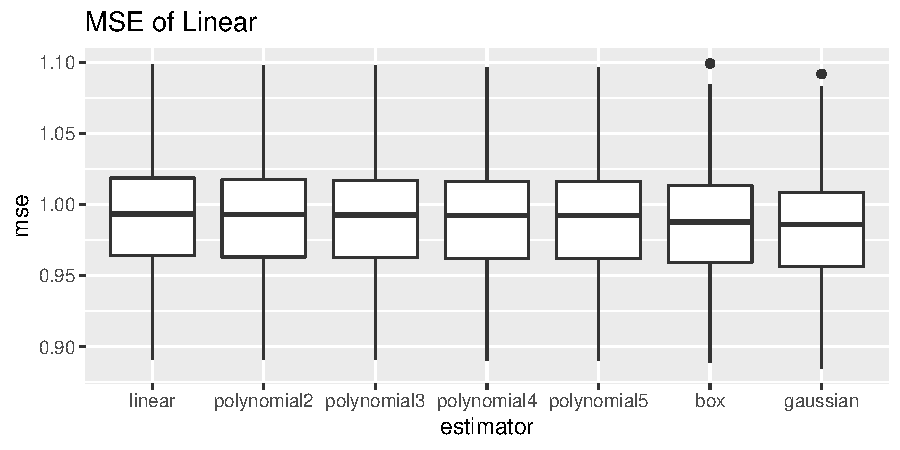
\includegraphics{mse_linear.pdf}
  \end{figure}
\item $f(x) = \sin(\pi x)$
    \begin{figure}[h]
      \centering
      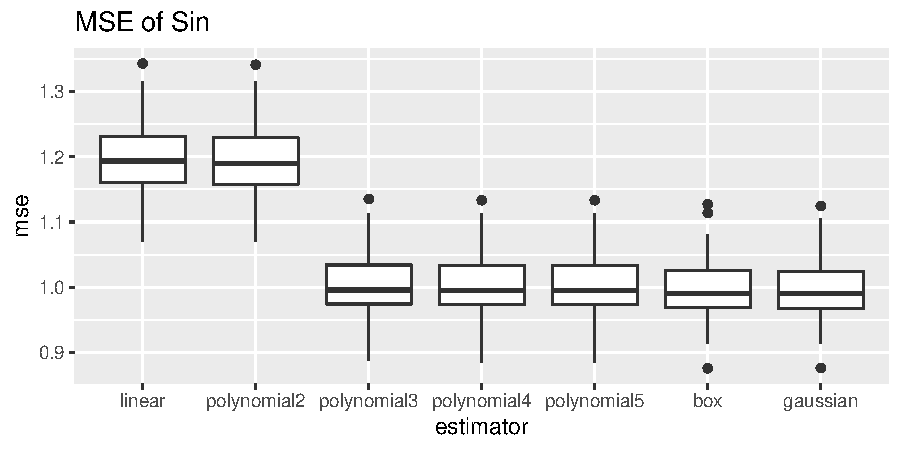
\includegraphics{mse_sin.pdf}
    \end{figure}
    \pagebreak
  \item $f(x) = 2x + x^3 - 6x^4$
    \begin{figure}[h!]
      \centering
      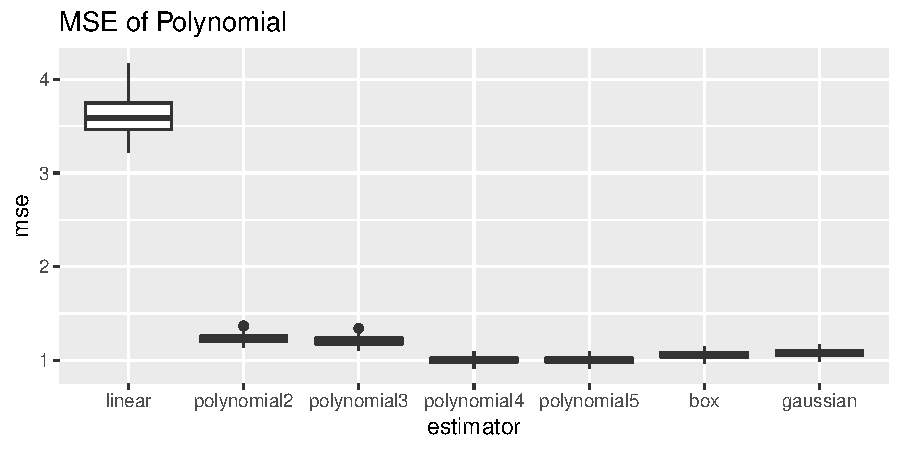
\includegraphics{mse_polynomial.pdf}
    \end{figure}

  \item $f(x) = 1/\left(1 + (5x)^2\right)$
    \begin{figure}[h!]
      \centering
      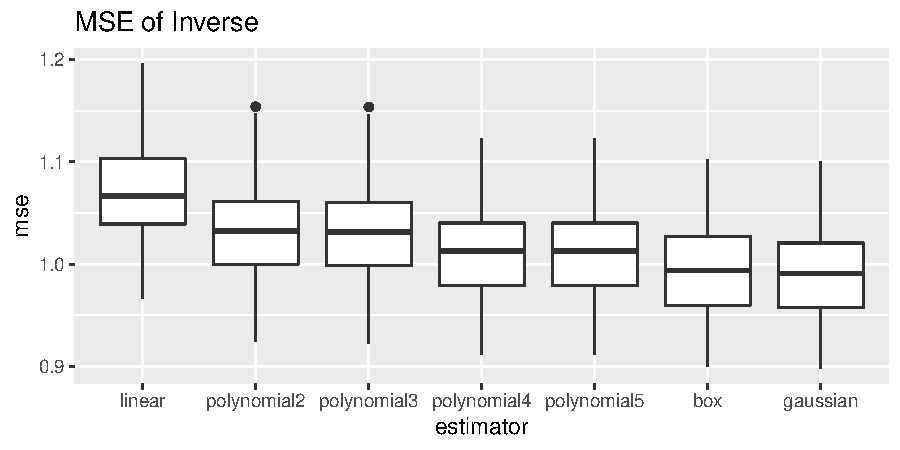
\includegraphics{mse_inverse.pdf}
    \end{figure}
  \end{enumerate}

  $n = 1000$ and 100 simulations were run for each case. Almost all the
  estimators achieve the optimal MSE of 1 when $f$ is linear.

  When $f$ is sinusoidal, the linear and degree 2 polynomial can no longer model
  the data.

  When $f$ is a higher-degree polynomial, the linear estimator does
  terribly. Unsuprisingly, the degree 4 and degree 5 polynomials do the best.

  When $f$ is an inverse polynomial function, increasing the degree of the
  polynomial estimator helps, but only the non-parametric models are able to
  achieve the theoretical best error of 1.
\end{document}
